\documentclass[12pt,letterpaper,noanswers]{exam}
\usepackage[usenames,dvipsnames,svgnames,table]{xcolor}
\usepackage[margin=0.9in]{geometry}
\renewcommand{\familydefault}{\sfdefault}
\usepackage{multicol}
\pagestyle{head}
\header{AM 22b Spring 2021}{Updated \today.}{Skill List for Skill Checks}
\runningheadrule
\headrule
\usepackage{graphicx} % more modern
\usepackage{amsmath} 
\usepackage{amssymb} 
\usepackage{hyperref}
\usepackage{tcolorbox}
\newcommand{\mb}[1]{\underline{#1}}
\usepackage[numbered,autolinebreaks,useliterate]{mcode}



\begin{document}
 \pdfpageheight 11in 
  \pdfpagewidth 8.5in

This document list 34 skills associated with content of the course.  A maximum of one skill is assigned per class meeting.  Skills are drawn from techniques and concepts that are either central to the course or that were challenging for students on past assessments.

\tableofcontents
  
\section{Functions, vectors, and derivatives}

\subsection{expression for the distance between a point and a plane parallel to the $xy$-, $xz$-, or $yz$-plane}

\noindent\textbf{Question}

Find an expression for the distance between the point $(a,b,c)$ and the plane $y = 7.$

\emph{You'll be given a point and a plane of the form $x = k$ or $y = k$ or $z = k$ where $k$ is a constant).}

\noindent\textbf{Solution}

Points in the plane are of the form $(x,7,z)$ for any $x,z\in \mathbb{R}$.  

The distance between $(a,b,c)$ and an arbitrary point in the plane is given by \[\sqrt{(a-x)^2 + (b-7)^2 + (c-z)^2}.\]

The distance between the point and the plane is defined as the minimum of all possible distances between the point and a point in the plane.  

$x$ and $z$ are arbitrary, and we choose them so as to find this minimum distance.  $(a-x)^2$ is non-negative, so its minimum is zero (at $x=a$).  Similarly for $(c-z)^2$.  The distance is $\sqrt{(b-7)^2}$.

The distance can be written as $\vert b-7\vert$ or as $\sqrt{(b-7)^2}$.  The expression $b-7$ would not be correct because it may have a negative value.


\subsection{find a level surface of a function of three variables}

\noindent\textbf{Question}

Find an expression for a level surface of the function \[f(x,y,z) = \ln{(x^2+3z^2)}.\]

Is the level surface a 

\begin{oneparcheckboxes}
\choice plane
\choice sphere or ellipsoid
\choice circular or elliptical paraboloid
\choice cylinder
\end{oneparcheckboxes}



\vspace{0.2cm}\noindent\textbf{Solution}


I set $\ln(x^2 + 3z^2) = c$.  Using $e$ to invert $\ln$, I have $x^2+3z^2 = e^c$.  Choose $c = 0$ as a convenient value to construct a single level surface, with $e^0 = 1$.  I have $x^2 + 3z^2 =1$ as an expression for one level surface of $f(x,y,z)$.

\begin{itemize}
    \item There are quadratic monomials in the level surface equation, so this isn't the equation for a plane.
    \item For a sphere or ellipsoid we would have $x^2$, $y^2$, $z^2$ all showing up, but we're missing $y^2$.
    \item Paraboloids are linear in one variable and quadratic in the other two, so the surface isn't a paraboloid.
    \item $y$ is missing from the expression, so this level surface will be a cylinder.  It is specifically an elliptical cylinder.
\end{itemize}


\subsection{rewrite the equation of a plane in two ways}

\noindent\textbf{Question}


Rewrite the equation of the plane
\[3x -5y +2z = 10 \]
\begin{itemize}
\itemsep0em
    \item in intercept form.
    \item using a dot product between a normal vector and a vector parallel to the plane.
\end{itemize}

\noindent\textbf{Solution}

For intercept form, I want $x/a + y/b + z/c = 1$ where $a, b, c$ are the axis intercepts of the plane.

Option 1: I'll divide by $10$ to make the right hand side $1$.  I have $3x/10 - y/2 + z/5 = 1$.  Rearranging, this is $\dfrac{x}{10/3} + y/(-2) + z/5 = 1$.

Option 2: I'll find the intercepts.  At $(a,0,0)$ we have $3a = 10$, so $a = 10/3$.  At $(0,b,0)$ we have $-5b = 10$ so $b = -2$.  At $(0,0,c)$ we have $2c = 10$ so $c=5$.  In intercept form the plane is \[\frac{x}{10/3}+\frac{y}{-2}+\frac{z}{5} = 1.\]

For the dot product, I can ``read'' the normal vector off of the plan equation.  It is $\langle 3,-5,2\rangle$.  To form a vector parallel to the plane, I use $(x,y,z) - (x_0,y_0,z_0)$, where $(x,y,z)$ is a variable point in the plane and $(x_0,y_0,z_0)$ needs to be a specific point in the plane.  The equation of the plane will be $\langle 3,-5,2\rangle \cdot \langle x-x_0,y-y_0,z-z_0\rangle = 0$, where $(x_0,y_0,z_0)$ is a point on the plane.  From the intercept form, we know that $(0,0,5)$ is a point on the plane, so one way to write the equation of the plane is
\[\langle 3,-5,2\rangle \cdot \langle x,y,z-5\rangle = 0.\] Of course, 
$\langle 3,-5,2\rangle \cdot \langle x,y+2,z\rangle = 0$ works as well.  As do many other options.  (So long as the point $(x_0,y_0,z_0)$ satisfies $3x_0 - 5y_0 +2z_0 - 10 = 0$, we will end up with a plane equation equivalent to $3x-5y+2z=10$.)


\subsection{compute a cross product}

\noindent\textbf{Question}

\begin{questions}
\item Let $\mb{u}$ be the vector 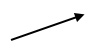
\includegraphics[scale=0.5]{img/C06p1a.png} and $\mb{v}$ be the vector 
\includegraphics[scale=0.5]{img/C06p1b.png}.

Is $\mb{u}\times\mb{v}$ into the page/screen (away from you) or out of the page/screen (towards you)?

\begin{oneparcheckboxes}
\choice into the page
\choice out of the page
\end{oneparcheckboxes}

\item Compute $(2\mb{i}+\mb{j})\times(2\mb{j})$ \textbf{using distributive and scalar multiplication properties} of the cross product along with the cross product relationships between $\mb{i},\mb{j},\mb{k}$.

\framebox(250,30){ cross product:\hfill }
\end{questions}

\noindent\textbf{Solution}

\begin{questions}
\item Two options for finding the direction using the right hand rule: 
\begin{itemize}
    \item Draw 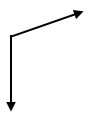
\includegraphics[scale=0.5]{img/C06p1c.png}.  Make a flat hand.  Leave your thumb and index (pointer) finger in place.  Bend your other three fingers towards your palm.  Rotate your hand to align the index finger with the first vector ($\mb{u}$) in such a position that you can also align the other fingers with ($\mb{v})$.  Which way is your thumb pointing?
    \item Draw 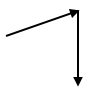
\includegraphics[scale=0.5]{img/C06p1d.png}, with $\mb{u}$ first and $\mb{v}$ drawn from its tip.  Place your palm along $\mb{u}$ oriented so that you can bend your fingers to align with $\mb{v}$.  Which way is your thumb pointing?
\end{itemize}
Your thumb should be into the page/screen in both cases.


    \item Distribute: \begin{align*}
    (2\mb{i}+\mb{j})\times(2\mb{j}) &= (2\mb{i})\times(2\mb{j})+ (\mb{j})\times(2\mb{j}) \\
    &= 4(\mb{i}\times \mb{j})+ 2(\mb{j}\times \mb{j}) \\
    &= 4(\mb{i}\times \mb{j}) \\
    &= 4\mb{k}.
    \end{align*}
%     \item Use determinant notation: \begin{align*}\left\vert\begin{array}{c c c} \mb{i} & \mb{j} & \mb{k} \\ 2 & 2 & 0 \\ 0 & 2 & 0
%     \end{array}\right\vert &= \mb{i}\left\vert\begin{array}{c c}2 & 0 \\ 2 & 0
%     \end{array}\right\vert - \mb{j}\left\vert\begin{array}{c c}2 & 0 \\ 0 & 0
%     \end{array}\right\vert + \mb{k}\left\vert\begin{array}{c c}2 & 2 \\ 0 & 2
%     \end{array}\right\vert \\
%     &= \mb{i}\left(2(0)-0(2)\right)-\mb{j}\left(2(0)-0(0)\right)+\mb{k}\left(2(2)-2(0)\right) \\
%     &= 4\mb{k}
%     \end{align*}
% \end{itemize}
\end{questions}

\subsection{compute a scalar triple product}

\noindent\textbf{Question}

Compute the scalar triple product of $\mb{u} = \left(\begin{array}{c}1 \\ 3\\ 2\end{array}\right)$, $\mb{v} =\left(\begin{array}{c}0 \\ -1\\ 1\end{array}\right)$, $\mb{w}=\left(\begin{array}{c} 2 \\ 1\\ 0\end{array}\right)$ using a determinant.

\noindent\textbf{Solution}

We can compute either $\text{det}\left([\mb{u}\ \mb{v}\ \mb{w} ]\right)$ or $\text{det}\left(\left[\begin{array}{c}\mb{u}^T \\ \mb{v}^T \\ \mb{w}^T \end{array}\right]\right)$ (they will be equal).


I'll expand using the top row, so $+,-,+$.

\begin{align*}
    \text{det}\left(\begin{array}{c c c}1 & 3 & 2 \\ 0 & -1 & 1 \\ 2 & 1 & 0 \end{array}\right) &= (1) \left\vert \begin{array}{c c} -1 & 1 \\ 1 & 0\end{array}\right\vert- (3) \left\vert \begin{array}{c c} 0 & 1 \\ 2 & 0\end{array} \right\vert + (2) \left\vert \begin{array}{c c}0 & -1 \\ 2 & 1\end{array} \right\vert \\
    &= (1)(0-1) -3(0-2) +2(0+2) \\
    &= -1 +6 + 4\\
    &= 9.
\end{align*}

If I choose the middle row, I need to use $-,+,-$ rather than $+,-,+$:
\begin{align*}
\text{det}\left(\begin{array}{c c c}1 & 3 & 2 \\ 0 & -1 & 1 \\ 2 & 1 & 0 \end{array}\right) &= -(0) + (-1) \left\vert \begin{array}{c c} 1 & 2 \\ 2 & 0\end{array} \right\vert - (1) \left\vert \begin{array}{c c}1 & 3 \\ 2 & 1\end{array} \right\vert \\
    &=  -(0-4) -(1-6) \\
    &= 4 +5\\
    &= 9.
\end{align*}
Check in Matlab:
\begin{lstlisting}
det([1 3 2; 0 -1 1; 2 1 0])
\end{lstlisting}


\subsection{compute directional derivative}
\noindent\textbf{Question}


\begin{questions}
\item Compute the directional derivative of $f(x,y) = 3x^2y$ at $(1,0)$ in the direction of $\mb{u} = \langle 1,3\rangle$.
\item Find the maximum possible directional derivative at $(1,0)$ (choosing from any direction).
\end{questions}

\vspace{0.2cm}\noindent\textbf{Solution}

$Df = [6xy, 3x^2]$.  At $(1,0)$ this is $[0, 3]$.  Creating a unit vector in the direction of interest, $\hat{\mb{u}}=\mb{u}/\Vert\mb{u}\Vert = \left(\begin{array}{c} 1/\sqrt{10} \\ 3/\sqrt{10}\end{array}\right)$.

The directional derivative is $f_{\mb{u}} =[0, 3]\left(\begin{array}{c} 1/\sqrt{10} \\ 3/\sqrt{10}\end{array}\right) = 0(1/\sqrt{10}) + 3(3/\sqrt{10}) = 9/\sqrt{10}$.

The maximum possible directional derivative is $\Vert \nabla f \Vert = \Vert Df \Vert = 3.$

\subsection{find the equation of a tangent plane to a surface}

\noindent\textbf{Question}

Find the equation of a tangent plane to $x^2 +y^2 - z = 1$ at the point $(1,3,9)$.

\noindent\textbf{Solution}

$x^2 + y^2 - z = 1$ is of the form $F(x,y,z) = c$.

\begin{itemize}
    \item Option 1: rewrite this as $z = f(x,y)$, with the tangent plane calculated at $(1,3)$. I have $z = x^2+y^2 -1$.  
    
    The tangent plane is $z = f(1,3) + \left. f_x\right\vert_{(1,3)}(x-1) + + \left. f_y\right\vert_{(1,3)}(y-3)$.
    
    $f_x = 2x$, $f_y = 2y$.  The tangent plane is
    \[z = 9 + 2(x-1) + 6(y-3)\]
    \item Option 2: $F = x^2 + y^2 - z$, so $[DF] = (2x, 2y, -1)$.  The function has a single output, so the gradient is defined and it is $\mb{\nabla}F = (2x, 2y, -1)^T$.  
    
    The gradient vector evaluated at a point on the surface is normal to the tangent plane of $F(x,y,z) = c$ at that point.
    
    At $(1,3,9)$, $\left.\mb{\nabla}F\right\vert_{(1,3,9)} = (2, 6, -1)^T$ is a vector normal to the tangent plane and $(1,3,9)$ is a point on the plane.
    
    \[2(x-1) + 6(y-3) + -1(z-9) = 0\] is an equation for the tangent plane.
\end{itemize}


\subsection{compute a derivative / Jacobian}

\noindent\textbf{Question}

Construct $D \mb{f}$ for the function $\displaystyle\mb{f} =  \left(\begin{array}{c}xze^y \\ x^2 + xyz \end{array}\right)$.

\noindent\textbf{Solution}

$D \mb{f}$ is the Jacobian matrix.  The function has three inputs and two outputs, so the Jacobian will be a 2x3 matrix (two rows and three columns).  Finding the six partials, we have $D\mb{f} = \left(\begin{array}{c c c}ze^y & x z e^y & xe^y \\ 2x + yz & xz & xy \end{array}\right)$

\subsection{use the chain rule to evaluate a partial derivative}

\noindent\textbf{Question}
Let $z = f(x,y) = \ln(xy)$ with $x = u^2+v^2$ and $y = u^3v$.  Let $\displaystyle\underline{x} = \left(\begin{array}{c} x\\ y\end{array}\right)$ and $\displaystyle\underline{u} = \left(\begin{array}{c} u\\ v\end{array}\right)$. Find $\displaystyle\frac{\partial z}{\partial\underline{x}}$ and $\displaystyle\frac{\partial \underline{x}}{\partial\underline{u}}$.  Use the chain rule to find $\displaystyle\frac{\partial z}{\partial\underline{u}}$.  Evaluate it at $u = 2, v = 1$.

\noindent\textbf{Solution} 


$\displaystyle\frac{\partial z}{\partial\underline{x}} = Df = [f_x, f_y] = [1/x, 1/y]$.
\vspace{0.2cm}

$\displaystyle\frac{\partial \underline{x}}{\partial\underline{u}} = \left(\begin{array}{c c} x_u & x_v \\ y_u & y _v\end{array}\right) = \left(\begin{array}{c c} 2u & 2v \\ 3u^2v & u^3 \end{array}\right)$.
\vspace{0.2cm}

$\displaystyle\frac{\partial z}{\partial\underline{u}} = \frac{\partial z}{\partial\underline{x}}\frac{\partial \underline{x}}{\partial\underline{u}} = \left[\frac{2u}{x}+\frac{3u^2v}{y}, \frac{2v}{x}+\frac{u^3}{y}\right] = \left[\frac{2u}{u^2+v^2} + \frac{3u^2v}{u^3v}, \frac{2v}{u^2+v^2}+\frac{u^3}{u^3v}\right] $

\hfill$\displaystyle= \left[\frac{2u}{u^2+v^2} + \frac{3}{u}, \frac{2v}{u^2+v^2}+\frac{1}{v}\right]$
\vspace{0.2cm}

At $(2,1)$ this is $\displaystyle\left.\frac{\partial z}{\partial\underline{u}} \right\vert_{(2,1)} = \left[\frac{4}{5} + \frac{3}{2}, \frac{2}{5}+1\right] = \left[\frac{23}{10}, \frac{7}{5}\right]$




\section{Integration}

\subsection{identify the sign of an integral using symmetry}
\noindent\textbf{Question}
Let $D$ be the unit disk centered about the origin in $xy$-space.  Identify the sign of $\int_D xy\ dA$.
\begin{oneparcheckboxes}
\choice positive
\choice zero
\choice negative
\end{oneparcheckboxes}

\emph{See the beginning of the problems section in \S 16.1 for about sixteen more examples (odd numbered problems have answers at the end of the text).}


\noindent\textbf{Solution}
$xy$ will be positive in the first and third quadrants.  It will be negative in the second an fourth quadrants.  For every small box $\Delta A$ in the first quadrant (containing the point $(a,b)$), there is a corresponding small box in the second quadrant (containing point $(a,-b)$).  We have $f(a,b) = -f(a,-b)$, and the contribution of those two small boxes to the integral is equal and opposite.  We can make the same argument for the contributions of the third and fourth quadrants.

The integral will be zero due to this symmetry.

\subsection{reverse the order of integration in a double integral}
\noindent\textbf{Question}
Reverse the order of integration for $\displaystyle\int_0^1\int_y^1 e^{x^2}\ dx\ dy$ and evaluate the integral.

\emph{See the problems section in \S 16.2 for six or so examples of this (odd numbered problems have answers at the end of the text).}

\noindent\textbf{Solution}

Start by drawing the region of integration based on the information in the bounds of the integral.

$x=y$ is the left bound for $x$ and $x=1$ is the right bound for $x$.  $y = 0$ is the bottom bound for $y$ and $y = 1$ is the top bound for $y$.

\begin{lstlisting}
syms x y
fimplicit(@(x,y) x-y) % plot x = y, or x - y = 0.
hold on
fimplicit(@(x,y) x-1) % plot x = 1, or x - 1 = 0.
fimplicit(@(x,y) y-0) % plot y = 0
fimplicit(@(x,y) y-1) % plot y = 1, or y - 1 = 0.
axis([-0.5 1.5 -0.5 1.5])
axis equal
xlabel('x'); ylabel('y');
\end{lstlisting}

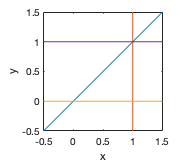
\includegraphics{img/C12-2dregion.png}

Construct the integral in the new order:
\begin{itemize}
\itemsep0em
    \item The inner integral is now with respect to $y$.  $y$ starts at $0$ for all values of $x$ and goes up to the line $x - y = 0$, so the line $y = x$.  
    \item The outer integral is with respect to $x$.  The `shadow' of the region on the $x$-axis is from $0$ to $1$.
    \item The function of integration (the integrand) does not change: $\displaystyle\int_0^1\int_0^x e^{x^2}\ dy\ dx$
\end{itemize}
\begin{align*}
    \int_0^1\int_0^x e^{x^2}\ dy\ dx &= \int_0^1\left[y e^{x^2}\right\vert_{y=0}^{y=x}\ dx \\
    &= \int_0^1 x e^{x^2}\ dx. \\
    \text{Let }u=x^2. & du = 2xdx\\
    \int_0^1\int_0^x e^{x^2}\ dy\ dx &= \int_{u=0^2}^{u=1^2} \frac{1}{2}e^u \ du \\
    &= \left[ \frac{1}{2}e^u\right\vert_0^1 \\
    &= \frac{1}{2}(e - 1).
\end{align*}


\subsection{sketch a cross-section of the region of integration for cylindrical coordinates}
\noindent\textbf{Question}
(cylindrical coordinates) Sketch the region in $rz$-space associated with the region of integration in the integral below and describe the shape of the region.
\[\int_0^{2\pi}\int_0^{1/\sqrt{2}}\int_0^z rz\ dr\ dz\ d\theta.\]

\noindent\textbf{Solution}


\begin{lstlisting}
syms r z
fimplicit(@(r,z) r)
hold on
fimplicit(@(r,z) r-z)
fimplicit(@(r,z) z)
fimplicit(@(r,z) z-1/sqrt(2))
axis equal
fill([0, 0,1/sqrt(2)],[0,1/sqrt(2),1/sqrt(2)],'r')
xlabel('r'); ylabel('z');
axis([0 1 -0.2 1])
\end{lstlisting}

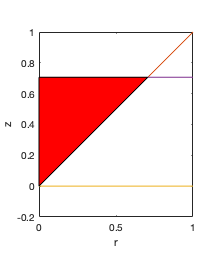
\includegraphics[scale=0.8]{img/C13skill.png}

The region is a solid cone.  (Imagine spinning this triangle around the $z$-axis through the angles $0$ to $2\pi$ to form the solid region).

\subsection{sketch a cross-section of the region of integration for spherical coordinates}
(spherical coordinates) Sketch the region in $rz$-space associated with the region of integration in the integral below and describe the shape of the region.
\[\int_0^{2\pi}\int_0^{\pi/4}\int_0^{\frac{1}{\sqrt{2}\cos\phi}} \rho^3\sin\phi\cos\phi\ d\rho\ d\phi\ d\theta.\]

\noindent\textbf{Solution}

The shape in $rz$-space is set by the $\rho$ and $\phi$ coordinates.  $\theta$ then rotates the shape we find about the $z$-axis.  Translating from spherical to cylindrical will allow us to find the $rz$ shape.

We have $\rho = 0$ and $\rho = \frac{1}{\sqrt{2}\cos\phi}$ for our $\rho$ bounds, where $\rho = 0$ is the origin, and $\rho\cos\phi = \frac{1}{\sqrt{2}}$ can be rewritten in cylindrical coordinates as $z = \frac{1}{\sqrt{2}}$.

The $\rho$ limits tell us that we have lines radiating from the origin that extend until $z = \frac{1}{\sqrt{2}}$.

For $\phi$, we have $\phi = 0$ as the lower bound.  This is the positive $z$-axis.  And we have $\phi = \pi/4$ as the upper bound.  This is a $45$-degree line in the $rz$-plane.

The $\phi$ bounds tell us that the radial lines from $0$ to $z=1$ are part of our region when they are between the positive $z$-axis and the $45$-degree line.

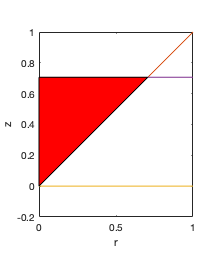
\includegraphics[scale=0.5]{img/C13skill.png}

The region is a solid cone.  (Imagine spinning this triangle around the $z$-axis through the angles $0$ to $2\pi$ to form the solid region).

\subsection{set up a double integral to find a probability}
\noindent\textbf{Question}
 Let $p$ be the joint probability density function such that $p(x,y) = xy$ in the rectangle $R$ where $0\leq x \leq 2, 0\leq y\leq 1$.  $p(x,y) =0$ outside of the rectangle.  Set up an integral to find the fraction of the population such that $x+y \leq 2$.
 
\noindent\textbf{Solution}
The probability that $x+y \leq 2$ is given by $\int_S p(x,y)\ dA$ where $S$ is the region of $R$ in which $x+y\leq 2$.  $R$ is shown in blue, with $S$ plotted on top of it in red 

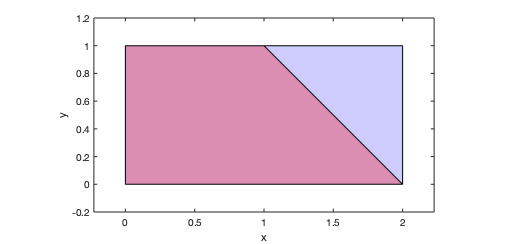
\includegraphics[width=3in]{img/C15skillcheck.png}

Setting up the integral:
\begin{align*}
   \int_0^1 \int_0^{2-y}xy\ dx\ dy
\end{align*}
If you were to integrate, you would find that the probability that $x+y\leq 2$ is less than half.

\subsection{read integration information from Matlab code}
\noindent\textbf{Question}
Based on the following code, identify (1) the rectangular box being used to enclose the region of integration, $R$, and (2) the region of integration.

\begin{lstlisting}
fc = @(x,y) x.*y;
npoints = 100000;
xyvals = rand(npoints,2)*2;
indomain = (xyvals(:,1).^2+xyvals(:,2).^2)<4; %set to 1 if in domain; 0 if not
sum(fc(xyvals(:,1),xyvals(:,2)).*indomain)*4/npoints
\end{lstlisting}

\noindent\textbf{Solution}

(1) The random numbers are generated in the interval $[0,2]$ (see line 3), so the rectangular box is $0\leq x \leq 2, 0\leq y \leq 2$.

(2) The region of integration comes from line 4: $x^2+y^2 < 4$ (and we have $x,y\geq 0$).  The region is the quarter disk in the first quadrant of the $xy$-plane.

\section{Vector calculus}

\subsection{provide a parameterization of a circle that meets the given conditions}
\noindent\textbf{Question}

(parameterization of a circle). Provide a parameterization for a circle of radius $2$, centered at $(1,5)$, and traversed counterclockwise.  Traverse the circle once.  Choose a parameterization so that the traversal takes time $20$.

\noindent\textbf{Solution}

One way to parameterize a circle is by using a variation on polar coordinates.  The circle is of radius $2$, so set $x(t) = 2\cos t$ and $y(t) = 2\sin t$.  This circle is centered at $(0,0)$ and it takes time $2\pi$ to traverse it.  The traversal direction (as $t$ increases) is counterclockwise.

Now make some adjustments: first shift the center of the circle.  Let $x(t) = 1+2\cos t$ and $y(t) = 5 + 2\sin t$.  The center of the circle has been shifted to $(1,5)$.

Next adjust the traversal time.  We want the input to $\sin$ and $\cos$ to be $2\pi$ when $t = 20$.  Write $x(t) = 1+2\cos kt$ and $y(t) = 5+2\cos kt$.  At time $t=20$ we want $kt = 2\pi$.  So $20k = 2\pi$ and $k = 2\pi/20 = \pi/10$.

Our parameterization of the circle is

$x(t) = 1+2\cos(\pi t/10)$ and $y(t)=5+2\sin(\pi t/10)$, $0\leq t\leq 20$.

Notice that I have included the time range in my answer (so that we traverse the circle exactly once).


\subsection{find the velocity along a parameterized curve}
\noindent\textbf{Question}

(velocity) Find $\mb v(t)$ for $\mb{r}(t) = t\mb i + t^2\mb j + t^3\mb k$.

\noindent\textbf{Solution}

$\mb v(t) = \frac{d\mb r}{dt} = \langle 1,2t,3t^2\rangle$.

\subsection{Identify the orientation and length of vectors in a vector field}
\noindent\textbf{Question}

\begin{questions}
\question Assume $x,y>0$.  For $\mb F = x\mb j$, decide if
\begin{parts}
\item the vectors in the vector field are

\begin{oneparcheckboxes}
\choice parallel to the $x$-axis
\choice parallel to the $y$-axis
\choice neither
\end{oneparcheckboxes}
\part As $x$ increases the length of the vectors

\begin{oneparcheckboxes}
\choice increases
\choice decreases
\choice neither
\end{oneparcheckboxes}

\part As $y$ increases the length of the vectors

\begin{oneparcheckboxes}
\choice increases
\choice decreases
\choice neither
\end{oneparcheckboxes}
\end{parts}
\end{questions}

\noindent\textbf{Solution}

\begin{questions}
\question 
\begin{parts}
\item The vector field is $\langle 0, x\rangle$ so vectors are parallel to the $y$-axis.
\item As $x$ increases $\Vert \mb F \Vert = \vert x \vert$ also increases.
\item As $y$ increases $\Vert \mb F \Vert = \vert x \vert$ does not change, so neither increases nor decreases.
\end{parts}
\end{questions}

\subsection{check whether parameterized curves are flow curves of a system of differential equations}
\noindent\textbf{Question}

\begin{questions}
\question For $\mb v = x\mb i + y\mb j$,
\begin{parts}
\item find the system of differential equations associated with the vector field.
\item Does the flow $x(t) = ae^t, y(t) = be^{-t}$ satisfy the system?  \emph{Show your calculation steps}

\begin{oneparcheckboxes}
\choice yes
\choice no
\end{oneparcheckboxes}
\end{parts}
\end{questions}


\noindent\textbf{Solution}

\begin{questions}
\question 
\begin{parts}
\item $\frac{dx}{dt} = x, \frac{dy}{dt} = y$.
\item $x(t) = ae^t$ so $\frac{dx}{dt} = ae^t$.  Does this satisfy $\frac{dx}{dt} = x$?  Yes: $ae^t=ae^t$.  $y(t) = be^{-t}$ so $\frac{dy}{dt} = -be^{-t}$.  Does this satisfy $\frac{dy}{dt}$?  No: $be^{-t} \neq -be^{-t}$.
\end{parts}
\end{questions}


\subsection{determine the sign of a line integral based on a diagram}
\noindent\textbf{Question}

Is the sign of the line integral for the pictured vector field and given curve to be positive, negative, or zero?

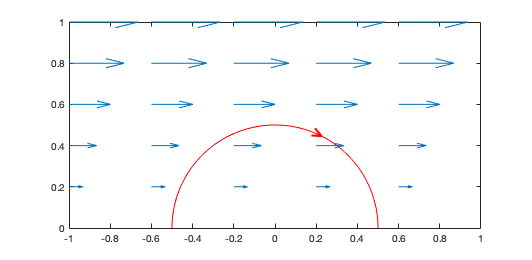
\includegraphics[width=4in]{img/C21lineintegral-p1.png}

\begin{oneparcheckboxes}
\choice positive
\choice negative
\choice zero
\end{oneparcheckboxes}

\noindent\textbf{Solution}

The angle between the velocity vector direction and the vector field is less than $\pi/2$ at every point, so the dot product that contributes to the line integral will always be positive.  That means we are integrating a positive function, so the integral will be positive.

\subsection{compute a line integral along a straight line path}
\noindent\textbf{Question}

Find $\displaystyle\int_C \mb F\cdot d\mb r$ for $\mb F = x^3\mb i + y^2\mb j + z\mb k$ and $C$ the line from the origin to the point $(2,3,4)$.




\noindent\textbf{Solution}

Parameterizing a line segment.  I'll use $0\leq t \leq 1$.  So $x(t) = 2t$, $y(t) = 3t$, $z(t) = 4t$.

\begin{align*}
\int_C \mb F \cdot \mb r &= \int_0^1 \langle (2t)^3, (3t)^2, (4t)\rangle \cdot \langle 2,3,4\rangle dt \\
&= \int_0^1 16t^3 + 27t^2 + 16t\ dt \\
& = \left. 4t^4 + 9t^3 + 8t^2 \right\vert_0^1 \\
& = 4 + 9 + 8 \\
&= 21.
\end{align*}


\subsection{use the fundamental theorem of calculus for line integrals}
\noindent\textbf{Question}


Let $f = x^2y$ and $\mb F = \nabla f.$  Let $C$ be a path connecting $(0,0)$ to $(1,4)$.  Use the ftcli to find $\int_C \mb F \cdot d\mb r$.



\noindent\textbf{Solution}


The ftcli says $\int_C \nabla f \cdot d\mb r = f(Q) - f(P)$ where path $C$ starts at point $P$ and ends at point $Q$.  We have $P = (0,0)$ and $Q = (1,4)$.  So $\int_C \nabla f \cdot d\mb r = 1^2(4)-0^2(0) = 4$.


\subsection{determine whether a vector field is irrotational}
\noindent\textbf{Question}

Find the scalar curl for $\mb F = \langle y, xy \rangle$.  Then identify whether $\mb F$ is an irrotational vector field, or not.

\noindent\textbf{Solution}

$Q = xy$, $P = y$.  $Q_x = y$.  $P_y = 1$.  $Q_x - P_y = y-1$.
The scalar curl is $y-1$, which is sometimes nonzero, so $\mb F$ is not irrotational.  

\subsection{use Green's theorem to convert from a line integral to an iterated integral}
\noindent\textbf{Question}

Let $C$ be the unit circle, traversed counterclockwise.  Use Green's theorem to set up an iterated integral to find $\displaystyle\oint_C x^2 dx + xydy$.

\noindent\textbf{Solution}

$mb F = \langle x^2, xy\rangle$, so $P = x^2, Q = xy$.  $Q_x = y, P_y = 0$.  The scalar curl is $Q_x - P_y = y$.  In polar, this is $r\sin\theta$.  The curve $C$ is oriented counterclockwise, so Green's theorem directly applies.  Integrate over the unit disk: $\displaystyle\int_0^{2\pi}\int_0^1 r\sin\theta\ rdrd\theta = \displaystyle\int_0^{2\pi}\int_0^1 r^2\sin\theta\ drd\theta$.

\subsection{given an oriented plane and vector field information, identify the sign of the flux}
\noindent\textbf{Question}

Identify the sign of the flux of $\mb F = x\mb j$ through the surface $S$, where $S$ is the piece of the plane $y = 2$ with $-3\leq x \leq 0, 0\leq z\leq 2$ and $S$ is oriented with its normal vector pointing towards the $xz$-plane.  Provide brief justification.

\noindent\textbf{Solution}


On the region $S$, $x\mb j$ points in the negative $\mb j$ direction because $x \leq 0$.

$S$ is a piece of the plane $y = 2$ so its normal vector is $\mb j$ or $-\mb j$.

We've been told to orient $S$ so that the normal vector points towards the $y = 0$ plane, so $-\mb j$.

The vector field and the normal vector are pointing in the same direction.  The flux will be positive.

\subsection{set up an integral to compute the flux of a vector field through a surface}
\noindent\textbf{Question}

Set up an integral to compute the flux of $\mb F = \cos y\mb i + z\mb j + \mb k$ through $S$ where $S$ is oriented upward and is the part of the surface $z = x^2+2y$ above the region $0\leq x\leq 2, 0\leq y\leq 1$.

\noindent\textbf{Solution}

$f(x,y) = x^2+2y$ so $f_x = 2x$, $f_y = 2$.  The vector $\mb u = \langle -f_x, -f_y, 1\rangle$ is normal to $f$ and points upwards.  It is $\mb u = \langle -2x, -2, 1\rangle$.

The component of $\mb F$ pushing upwards through $z = f(x,y)$ is $\mb F \cdot \dfrac{\mb u}{\Vert \mb u \Vert}$.  On the surface, $\mb F = \cos y\mb i + (x^2+2y)\mb j + \mb k$, so $\mb F\cdot \mb u = -2x\cos y -2(x^2+2y) + 1$



We have 
\begin{align*}
\int_S \mb F\cdot d\mb A &= \int_S \mb F \cdot \dfrac{\mb u}{\Vert \mb u\Vert}dS \\
&= \int_R \mb F \cdot \dfrac{\mb u}{\Vert \mb u\Vert} \Vert\mb u\Vert dA \\
&= \int_R \mb F \cdot \mb u\ dA \text{ (you can jump straight to this expression)}\\
&= \int_0^1 \int_0^2 (-2x\cos y -2(x^2+2y) + 1) dx dy
\end{align*}

Recall that $S$ is the original surface (in $3$-space) and $R$ is its projection/shadow in the $xy$-plane.  In this problem, $R$ was specified in the problem statement. $dS$ is a tiny piece of $S$ while $dA$ is a tiny piece of $R$.  (But $d\mb A$ and $d\mb S$ are each used to refer to the area vector associated with a tiny piece of $S$).



\subsection{find the flux out of a closed surface (use the divergence theorem)}
\noindent\textbf{Question}


 Find the flux of $\underline F = (x+3e^{yz})\mb i + (\ln(x^2z^2+1)+y)\mb j + z\mb k$ out of the closed solid cylindrical region of radius $2$ centered on the $z$-axis, $0\leq r\leq 2$, $3\leq z \leq 7$.



\noindent\textbf{Solution}


Using the divergence theorem, $\nabla\cdot \underline F = 1 + 1 + 1 = 3$ so the flux is $\int_W 3dV = 3\int_W dV$.  
$3\int_W dV = 3\int_0^{2\pi}\int_0^2\int_3^7 rdzdrd\theta = 12\int_0^{2\pi}\int_0^2 rdr = 24\int_0^{2\pi}d\theta = 48\pi$

\subsection{orient surfaces of a solid object to match the divergence theorem}
\noindent\textbf{Question}

Consider a solid ball $W$.  Let $S_1$ be the surface of the upper half of the ball, oriented upwards.  Let $S_2$ be the surface of the lower half of the ball, also oriented upwards.  Provide an equation that relates $\displaystyle\int_{S_1}\mb F\cdot d\mb S,\int_{S_2}\mb F\cdot d\mb S,\int_{W}\nabla \cdot \mb F\ dV$.


\noindent\textbf{Solution}

The surface of $W$, $\partial W$, is oriented outwards, so $\partial W = S_1-S_2$.
By the divergence theorem, $\int_W \text{div }\mb F dV = \int_{S_1-S_2}\mb F\cdot d\mb S$.

We have $\displaystyle\int_W \text{div }\mb F\ dV = \int_{S_1}\mb F\cdot d\mb S-\int_{S_2}\mb F\cdot d\mb S$

\section{Differential equations}
\subsection{find equilibrium solutions to an autonomous first order differential equation}
\noindent\textbf{Question}

Find all solutions to $\frac{dx}{dt} = x(1-x)$ where $x(t) = c$ with $c$ a constant (these are all of the equilibrium solutions).

\noindent\textbf{Solution}

$\frac{dx}{dt} = x(1-x) = 0$ when $ x = 0 $ or $1 - x = 0$ so $x(t) = 0$ is an equilibrium solution and $x(t) = 1$ is an equilibrium solution.


\subsection{classify the stability of equilibrium solutions}

\noindent\textbf{Question}

Classify the stability of the equilibrium solutions of $\dfrac{dx}{dt} = x(1-x)(3-x)$.

\noindent\textbf{Solution}

\begin{enumerate}
    \item Find the equilibrium solutions: Equilibrium solutions when $\frac{dx}{dt} = 0$ for some $x$, so $x^* = 0, 1, 3$.
    \item To identify stability, check $f'(x^*)$.
    \item Using the product rule,
$\dfrac{df}{dx} = (1)(1-x)(3-x) + x(-1)(3-x) + x(1-x)(-1)$.
\item Substitute the different equilibrium solutions: 

Substituting $x^* = 0$, $f' = (1)(3) = 3$.  Unstable

Substituting $x^* = 1$, $f' = 1(-1)(2) = -2$.  Stable

Substituting $x^* = 3$, $f' = 3(-2)(-1) = 6$.  Unstable
\end{enumerate}

\subsection{use separation to find a solution to a simple diff eq}
\noindent\textbf{Question}


Show the mathematical steps to find a solution to $\frac{dx}{dt} = -4x, x(0) = 2$.


\noindent\textbf{Solution}


For the skill check, you'll need to show your mathematical steps but do not need to provide written descriptions of the steps.

\begin{enumerate}
    \item 'Separate' variables: $\frac{1}{x}\frac{dx}{dt} = -4$.
    \item Integrate both sides with respect to time.  $\displaystyle\int \frac{1}{x(t)}\frac{dx}{dt}dt = \int -4 dt$.
    \item Change variables on the left hand side: $u = x(t)$, 
    $du = \frac{dx}{dt}dt$.  
    $\int \frac{1}{u}du = -4t + C$
    \item Integrate the left hand side.  $\ln \vert u\vert = -4t + C$.
    \item Rearrange: $u = e^Ce^{-4t}$
    \item Return to the original variables: $x(t) = e^Ce^{-4t}$.
    \item Set $C$ so that $x(0) = 2$.  $x(0) = e^Ce^{0} = e^C = 2$.  $x(t) = 2e^{-4t}$. 
\end{enumerate}



\subsection{use separation to find a solution to an initial value problem}
\noindent\textbf{Question}

Find a family of solutions to the initial value problem $\dfrac{dx}{dt} = x^2t, x(1) = 1$.

\noindent\textbf{Solution}

Separating: $\dfrac{1}{x^2} \dfrac{dx}{dt} = t$.  Integrating with respect to $t$ (and changing the variable of integration on the left hand side) $\displaystyle\int \frac{1}{x^2} dx = \int t\ dt$.  $-\dfrac{1}{x} = \frac{1}{2}t^2 + c$, so $x(t) = \dfrac{1}{t^2/2 + c}$.  $x(1) = 1$ so $\dfrac{1}{1/2 + c} = 1$.  $c = 1/2$.  We have $x(t) = \dfrac{1}{t^2/2 + 1/2}$



\subsection{construct a phase portrait for an autonomous 1st order ODE}
\noindent\textbf{Question}

Sketch the phase portrait in phase space for $\dot x = x(1+x)(2+x)$.  (Construct the phase line)

\noindent\textbf{Solution}


$\dot x = 0$ for $x = 0, -1, -2$, so those are the locations with circles.

For $x > 0$, $\dot x = + + + > 0$ (the three terms of the product are each positive).

For $-1 < x < 0, \dot x = - + + < 0$.

For $-2 < x < -1, \dot x = - - + > 0$.

For $-2 < x, \dot x = - - - < 0$.

Drawing these arrows onto the line, and filling in the circle at $x = -1$, I have:


\includegraphics{img/C34skillex.pdf}

\subsection{convert a 2nd order ODE into a 1st order system}
\noindent\textbf{Question}

Rewrite the differential equation $2\ddot x + 7\sin t\dot x - 3x^2 = 0$ as a system of first order differential equations. 


\noindent\textbf{Solution}

Let $ y = \dot x$.  We have $\ddot x = \dot y = \frac{3}{2}x ^2- \frac{7\sin t}{2}\dot x = \frac{3}{2}x ^2- \frac{7\sin t}{2}y$.

The system should be written in terms of just $x,y,t$, and it is
$\displaystyle\left\{\begin{array}{l} \dot x = y \\ \dot y = \frac{3}{2}x^2 - \frac{7\sin t}{2}y
\end{array}\right.$


\end{document}